% vim: spelllang=fr

\documentclass[../main.tex]{subfiles}
\graphicspath{{\subfix{../Figures/Chap4/}}}
\begin{document}

\begin{itshape}
    Dans ce dernier chapitre, on établit et applique des indices de cyclogénèse, construits par régression de Poisson, non plus dans le monde de la réanalyse et
    des observations, mais dans le monde du modèle avec ARPEGE-Climat. L'ajout de nouveaux prédicteurs dans la régression est exploré, et une attention
    particulière est portée à la recherche de tendances à long terme. Les indices sont ensuite appliqués à des simulations à climat plus chaud avec ARPEGE
    utilisé dans sa configuration basculée-étirée sur les antilles et sur le bassin Sud-Indien.
\end{itshape}

\minitoc
\newpage

%--------------------------------------
\section{Introduction}

Dans le \cref{chap:chapitre_3}, nous avons construit des indices de cyclogénèse par régression de Poisson en prenant la réanalyse ERA5 comme source pour
l'environnement de grande échelle, et la base de données observationnelle IBTrACS comme référence pour les observations. Dans ce chapitre, nous nous
intéresserons à l'utilisation d'indices de cyclogénèse dans des simulations climatiques réalisées avec ARPEGE-Climat. [En cours]

Il faut justifier le fait de faire un indice de cyclogénèse sous perfusion Niño 3.4 pour essayer de donner de l'amplitude et de la corrélation à la variabilité
interannuelle. Si on demande, on le fait dans le monde du modèle parce que les travaux ERA5 sont plutôt une introduction aux outils et aux méthodes utilisées
pour les indices, notamment pour l'aspect validation de la reproduction de la méthodologie de Tippett, et la déclinaison en régression à l'échelle du bassin ;
indispensable pour Niño mais aussi pour les runs climat futur puisqu'elles sont faites en basculée-étirée.

\section{Utilisation d'un indice Niño dans une régression de Poisson}\label{sec:indice_ONI}

On s'intéresse ici à l'ajout explicite du signal du mode de variabilité ENSO (\textit{El Niño-Southern Oscillation}) dans un indice de cyclogénèse construit par
régression de Poisson. Il s'agit de voir si ce nouvel apport d'information est susceptible d'introduire de l'amplitude dans la variabilité interannuelle inférée
par un tel indice, et de voir si ce prédicteur peut, ou non, améliorer au moins localement la représentation de la variabilité interannuelle.

\subsection{Données et Méthodes}

\subsubsection{Simulation historique forcée avec ARPEGE-Climat}

Nous utilisons ici le modèle ARPEGE dans sa version 6.3 à haute résolution, dans la même configuration que dans
\textcite{chauvin_future_2020,cattiaux_projected_2020}. Cette version du modèle est quasiment identique à celle utilisée dans le modèle couplé CNRM-CM6-1
\parencite{voldoire_evaluation_2019} et CNRM-ESM2 \parencite{seferian_evaluation_2019}, participant à CMIP6 \parencite{eyring_overview_2016} et HighResMIP
\parencite{haarsma_highresmip_2020}. Une description détaillée de toutes les nouveautés dans cette version d'ARPEGE par rapport à la version précédente (5.2)
est disponible dans \textcite{voldoire_evaluation_2019}, tandis que la version précédente est décrite dans \textcite{voldoire_cnrmcm5_2013}. Nous ne précisons
alors ici que les éléments particulièrement pertinents pour la simulation des cyclones tropicaux. Ainsi, le modèle est constitué du schéma physique PCMT
(\textit{Prognostic Condensates Microphysics and Transport}), incluant le schéma convectif de \textcite{piriou_approach_2007,gueremy_continuous_2011}, offrant
une paramétrisation de la convection profonde et peu profonde. Cette version voit également l'ajout de dix nouvelles variables pronostiques\footnote{Les
variables dites \textquote{pronostiques} se distinguent des variables dites \textquote{diagnostiques} en cela que leur évolution temporelle est décrite par la
résolution d'une équation dans le modèle numérique. Par opposition, les variables diagnostiques (par exemple, l'humidité relative) sont dérivées des variables
pronostiques (température, pression, humidité spécifique...).}, en plus des six déjà présentes. Spécifiquement, ARPEGE 6.3 calcule désormais l'évolution du
contenu en eau liquide et solide, précipitée ou nuageuse, de l'énergie cinétique turbulente et de la vitesse verticale convective. La paramétrisation de la
microphysique provient du schéma de \textcite{lopez_implementation_2002}, tandis que le schéma de turbulence est issu de \textcite{cuxart_turbulence_2000}. Le
modèle possède \num{91} niveaux verticaux, jusqu'à \hPa{0.01}, et la couche de mélange atmosphérique est caractérisée par \num{15} niveaux verticaux en dessous
de \m{1500} d'altitude.

La simulation utilisée ici est une simulation historique sur la période \num{1979}~--~\num{2010} et sur une grille T359, de taille \num{720} (longitude)
$\times$ \num{360} (latitude), donc à une résolution horizontale de \ang{0.5}, soit d'environ \km{50} à l'équateur. La simulation est forcée par la SST et la concentration
en glace de mer issues d'observations et provenant de la base de données HadISST1 \parencite{rayner_global_2003}.

\subsubsection{Cylogénèses simulées}\label{sec:tracking_arpege}

Les cyclones tropicaux sont détectés à l'aide du schéma de détection du CNRM \parencite{chauvin_response_2006}, amplement décrit dans le \cref{chap:chapitre_2},
notamment dans la \cref{sec:eval_tracker_ERA5}. Le schéma de détection a été appliqué aux champs 6-horaires du modèle avec : un seuil de vorticité
\textbf{VOR}~$=$~\SI{20e-5}{\per\second} ; un seuil de vent \textbf{RES}~$=$~\ms{13}, un seuil d'anomalie de température \textbf{TANOM}~$=$~\SI{1}{\kelvin} ; un
seuil de profil vertical de température \textbf{PT}~$=$~\SI{-2}{\kelvin} ; un seuil de profil vertical de vitesse du vent \textbf{PW}~$=$~\ms{5}, et enfin un
paramètre de relaxation des trajectoires \textbf{REL} fixé à \SI{20e-5}{\per\second}. Ces paramètres se distinguent notablement de ceux utilisés pour ERA5 dans
\textcite{dulac_assessing_2023} par le seuil vorticité (respectivement \SI{15e-5}{\per\second}) et surtout par le seuil de vitesse du vent à la surface
(respectivement \ms{5}). Rappelons en effet que le modèle ARPEGE, en particulier cette version précise du modèle, est connue pour simuler des cyclones tropicaux
intenses par rapport à la résolution du modèle \parencite{roberts_impact_2020,chauvin_future_2020} (voir aussi \cref{sec:cyclones_dans_modèles} du
\cref{chap:chapitre_1}, notamment la \cref{fig:roberts_PV_resolution}, \vpageref{fig:roberts_PV_resolution}). Il convient néanmoins de préciser que
contrairement au \cref{chap:chapitre_2}, le choix des seuils de détection utilisés pour détecter les TC dans cette simulation n'ont pas fait l'objet d'une
analyse quantitative des performances ---~une telle analyse serait par ailleurs impossible étant donné qu'il n'existe pas de trajectoires de référence pour les
pures simulations atmosphériques. Avant post-traitement des trajectoires, la fréquence d'occurrence annuelle moyenne de cyclogénèses est de \num{80.7} TC par
an. À titre de référence, IBTrACS sur la même période indique \num{82.9} TC par an.

Nous appliquons en post-traitement le filtre des systèmes de moyennes latitudes basé sur le diagnostique du jet subtropical (STJ), décrit et illustré dans la
\cref{sec:filtrage_mid_latitudes} (\cref{chap:chapitre_2}). Ce filtre est choisi ici ---~en dépit des réserves exprimées dans le \cref{chap:chapitre_2}~--- en
raison de sa relative simplicité à implémenter, notamment par rapport au filtre du $V_U^T$ qui a lui été préféré dans \textcite{dulac_assessing_2023}. En effet,
l'emploi du filtre du $V_U^T$ comme post-traitement nécessite de traiter en profondeur les champs spatiaux 3D du modèle centrés sur les positions des TC
préalablement identifiés, une opération qui est à la fois techniquement complexe et chronophage. En comparaison, la détermination de la limite équatoriale du
STJ peut être faite une fois pour toutes, et n'est pas à proprement parler dépendante des trajectoires identifiées, au sens où il n'est pas nécessaire de
répéter le diagnostique pour appliquer le filtre à de nouvelles trajectoires issues de la même simulation. En outre, \textcite{bourdin_intercomparison_2022}
montrent que le filtre du STJ parvient très efficacement à filtrer les systèmes de moyennes latitudes, lorsqu'appliqué à plusieurs schémas de détection sur
ERA5. Rappelons brièvement que la latitude du STJ est déterminée en prenant la limite équatoriale des points où le module du vent à \hPa{200} (lissé sur trois
mois glissants) est supérieur à \ms{25} et où la composante zonale (lissée de la même façon) est supérieure à \ms{15}. En pratique, puisqu'on s'intéresse aux
cyclogénèses et qu'on ne garde pour cela que les premières échéances des trajectoires, le filtre consiste à retirer les points situés au delà de la latitude du
STJ.

La \cref{fig:track_density_PRE625REFT359x} présente la densité annuelle moyenne (sur \num{30} ans) des premières échéances des trajectoires détectées dans la
simulation ARPEGE ---~assimilées aux cyclogénèses~--- après application du filtre du STJ. Avec le filtre du STJ, la fréquence annuelle moyenne est réduite à
\num{60.8} TC par an. Le filtre retire en effet \num{617} cyclogénèses, mais tous ne sont pas purement extra-tropicaux car la latitude médiane des cyclogénèses
filtrées est de \ang{26.2}N dans l'hémisphère nord ($n = \num{366}$) et de \ang{31.8}S dans l'hémisphère sud ($n=251$). On note également une latitude minimale
parmi les systèmes filtrés à \ang{2}N et à \ang{8.6}S pour chacun des deux hémisphères respectifs. Le jet subtropical ne peut physiquement pas se trouver en
dessous de \ang{2}N. Ce cas illustre un des points (en l'occurence une des limitations du filtre) discuté dans la \cref{sec:filtrage_mid_latitudes} (et
parfaitement illustré sur la \cref{fig:geopdy_and_STJ}, troisième ligne, \vpageref{fig:geopdy_and_STJ}), et peut être considéré comme un effet de bord. Le
filtre parvient toutefois à supprimer \num{95} des \num{97} cyclogénèses situées au delà de \ang{40} (nord et sud) dans les trajectoires non-filtrées.

\begin{figure}[tb]
    \centering
    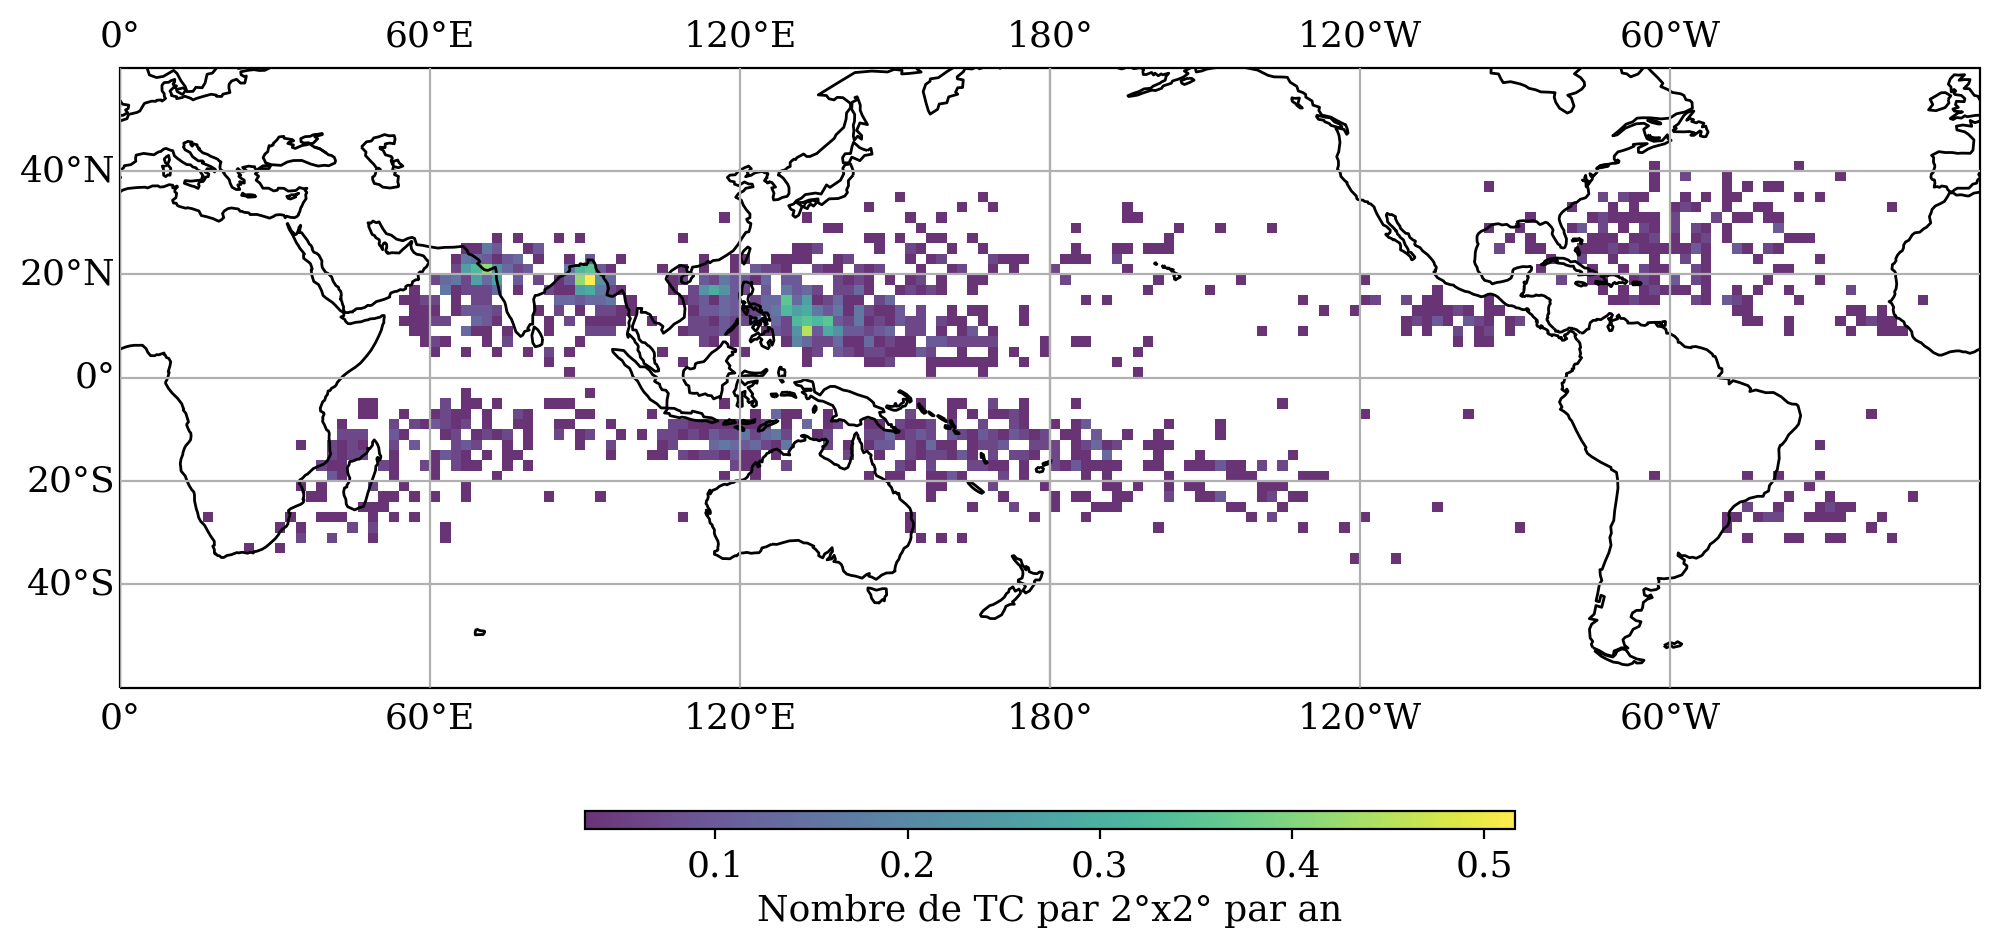
\includegraphics[width=\textwidth]{track_density_PRE625REFT359x.png}
    \caption{Densité annuelle moyenne de cyclogénèses dans la simulation ARPEGE forcée par HadISST1 entre 1980 et 2010, calculée sur une grille régulière de
    \ang{2}$\times$\ang{2}.}
    \label{fig:track_density_PRE625REFT359x}
\end{figure}

La \cref{fig:density_arpege_ibtracs} présente le biais moyen entre la simulation ARPEGE (c.f \cref{fig:track_density_PRE625REFT359x}) et IBTrACS, prise sur la
même période, en termes de densité de probabilité d'occurrence pour pallier à la différence dans la fréquence annuelle des deux jeux de données après
application du filtre du STJ. Dans l'océan Atlantique, la \cref{fig:density_arpege_ibtracs} fait apparaître une légère surestimation dans l'Atlantique sud d'une
part, et une déséquilibre dans l'Atlantique nord avec notamment une sous-évaluation dans le MDR et le GoM, mais une sur-évaluation dans le reste de l'océan. Ce
biais dans l'atlantique nord avec cette simulation est par ailleurs documenté dans \textcite{chauvin_future_2020}. Dans le bassin EPac, l'activité simulée est
fortement sous-estimée. Dans le WPac, un surplus est noté dans ARPEGE en Mer de Chine méridionale et Mer des Philippines, tandis que le reste du bassin voit
sinon un déficit. Dans le bassin NInd, la simulation ARPEGE présente une activité sur-estimée aussi bien en Mer d'Arabie que dans le Golfe du Bengale. Dans
l'hémisphère sud, le biais est plus contrasté. Dans l'océan Indien, on note un biais positif dans le sud-ouest du bassin, autour de Madagascar mais un biais
négatif dans le nord-est, proche de l'équateur. Une répartition du biais similaire mais symétrique est notée dans le bassin Sud Pacifique, avec un biais positif
dans le sud-est et négatif au nord-ouest.

Dans la plupart des bassins, ces motifs de biais sont en fait évocateurs d'une mauvaise localisation des cyclogénèses par le schéma de détection, notamment en
raison de sa tendance connue à détecter les TC un peu tardivement, plutôt que d'un biais avéré dans l'activité simulée. Dans le NAtl, les trajectoires démarrent
le plus souvent de la MDR ou du GoM pour ensuite remonter vers le nord / nord-est. Dans le SInd, les TC se déplacent souvent du nord-est vers le sud-ouest. La
sens de circulation est inversé dans le SPac en raison du flux de mousson en provenance d'ouest qui prend le pas sur la dérive de Coriolis ---~cette dernière
ayant naturellement tendance à déplacer les TC vers l'ouest dans l'hémisphère sud (c.f \cref{sec:conditions_cyclogenese})~--- si bien que les TC s'y déplacent
généralement vers le sud-est. Une détection trop tardive des TC pourrait également expliquer au moins en partie le biais noté dans le WPac (voir aussi
\cref{fig:bassins_TC} du \cref{chap:chapitre_1}, \vpageref{fig:bassins_TC}, pour voir les sens de déplacement des TC dans les bassins océaniques majeurs). Le
\cref{chap:chapitre_2} fait notamment référence à cette tendance que possède le schéma de détection à détecter trop tardivement les TC dans la réanalyse ERA5,
et cet effet est également documenté dans \textcite{bourdin_intercomparison_2022}. Dans ce contexte, les seules régions où il existe un biais réel entre
l'activité simulée par ARPEGE et l'activité observée (outre la différence de fréquence annuelle après passage du filtre) sont le bassin EPac, le NInd, et dans
une mesure bien moindre le Sud Atlantique. L'activité cyclonique telle que simulée dans le modèle ARPEGE et identifiée par le traqueur du CNRM est donc tout
compte fait assez fidèle aux observations. Nous considérons alors que les cyclogénèses issues du schéma de détection du CNRM appliqué à la simulation ARPEGE
peuvent être utilisées comme prédictant pour la construction d'indices de cyclogénèse par régression de Poisson.

\begin{figure}[tb]
    \centering
    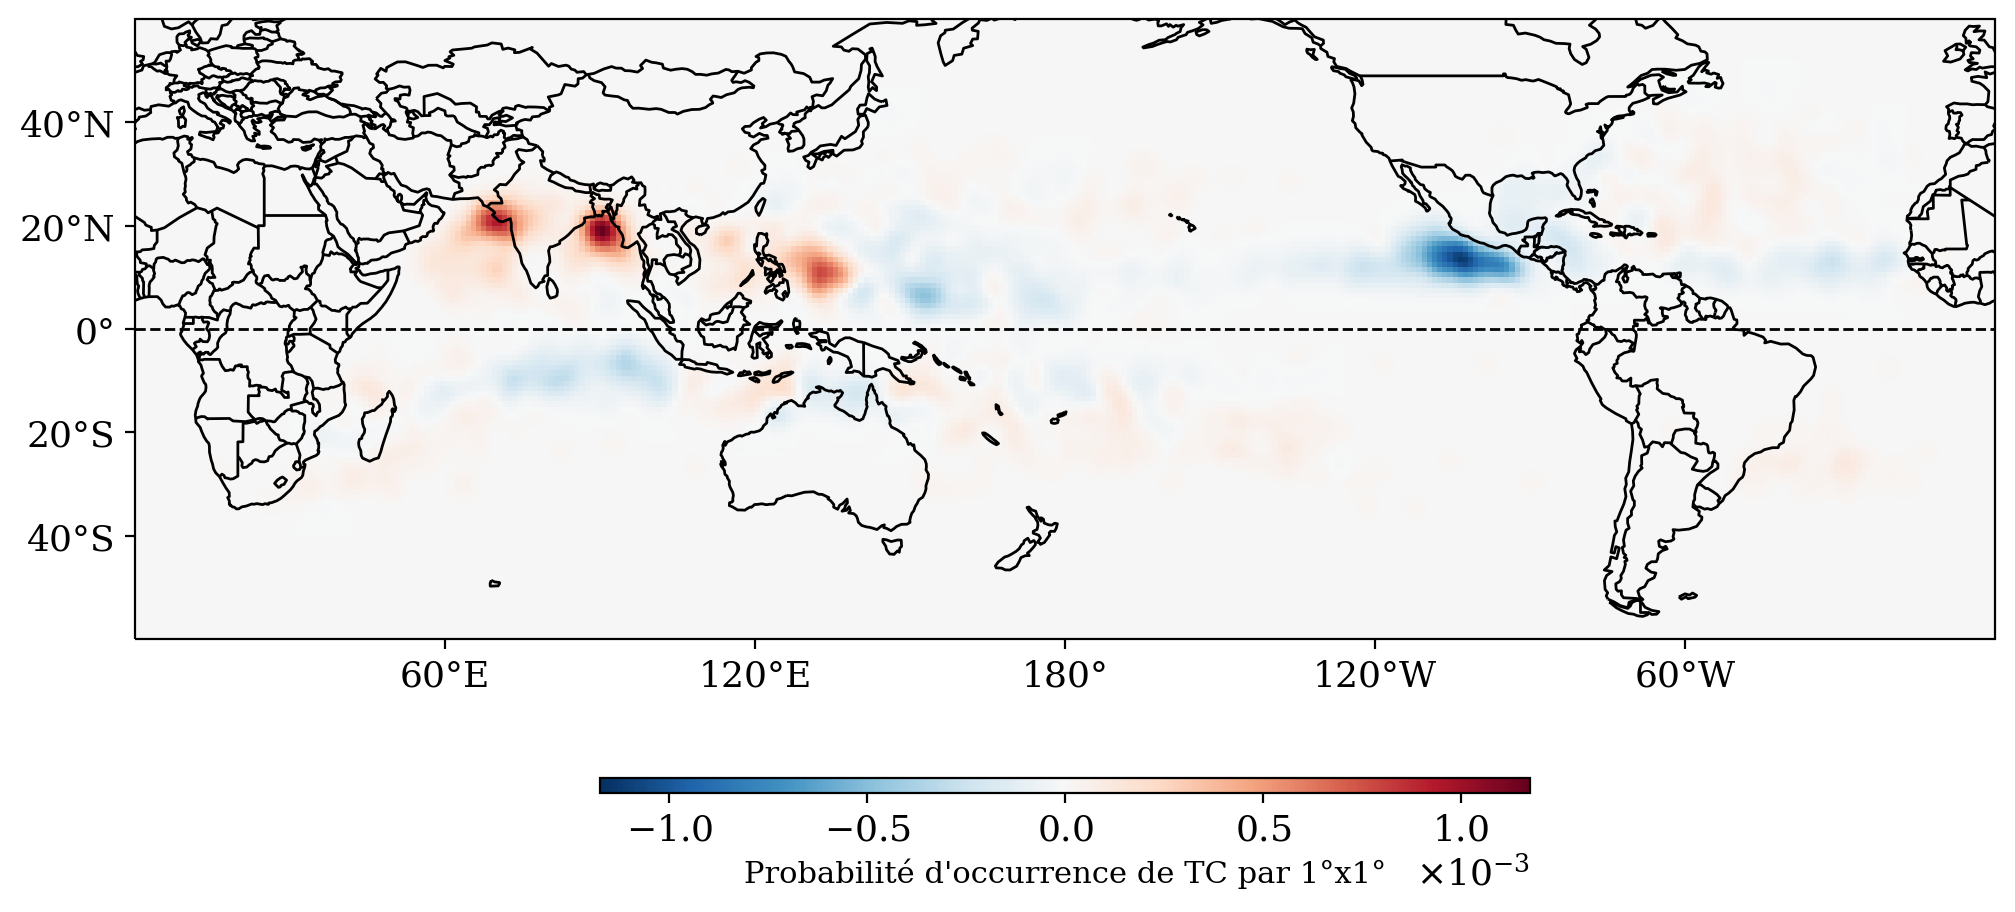
\includegraphics[width=\textwidth]{density_arpege_ibtracs.png}
    \caption{Carte de la différence entre les densités de cyclogénèses moyennes et normalisées ---~lissées au préalable avec un filtre gaussien à \ang{1}
    d'écart-type~--- de la simulation ARPEGE forcée et IBTrACS entre \num{1980} et \num{2010}.}
    \label{fig:density_arpege_ibtracs}
\end{figure}

%La \cref{fig:STJ_PRE625REFT359x} présente quant à elle les moyennes saisonnières de la latitude diagnostiquée par le filtre du STJ pour les deux hémisphères.
%Les variations saisonnières du STJ de la \cref{fig:STJ_PRE625REFT359x} illustrent le caractère dynamique du filtre du STJ, par rapport à une limite en latitude
%fixe. Cette figure met aussi en évidence le caractère saisonnier du filtre, avec un décalage vers les pôles durant les saisons chaudes, et un déport vers
%l'équateur durant la saison froide, les deux étant bien entendu en opposition de phase dans chacun des hémisphères. Cette propriété du seuil dynamique en
%latitude avait déjà été mise en évidence pour le filtre du gradient de géopotentiel à \hPa{200} présenté dans la \cref{sec:filtrage_mid_latitudes}
%(\cref{chap:chapitre_2}), mais n'avait pas été documentée pour le filtre du STJ.

%\begin{figure}[tp]
%    \centering
%    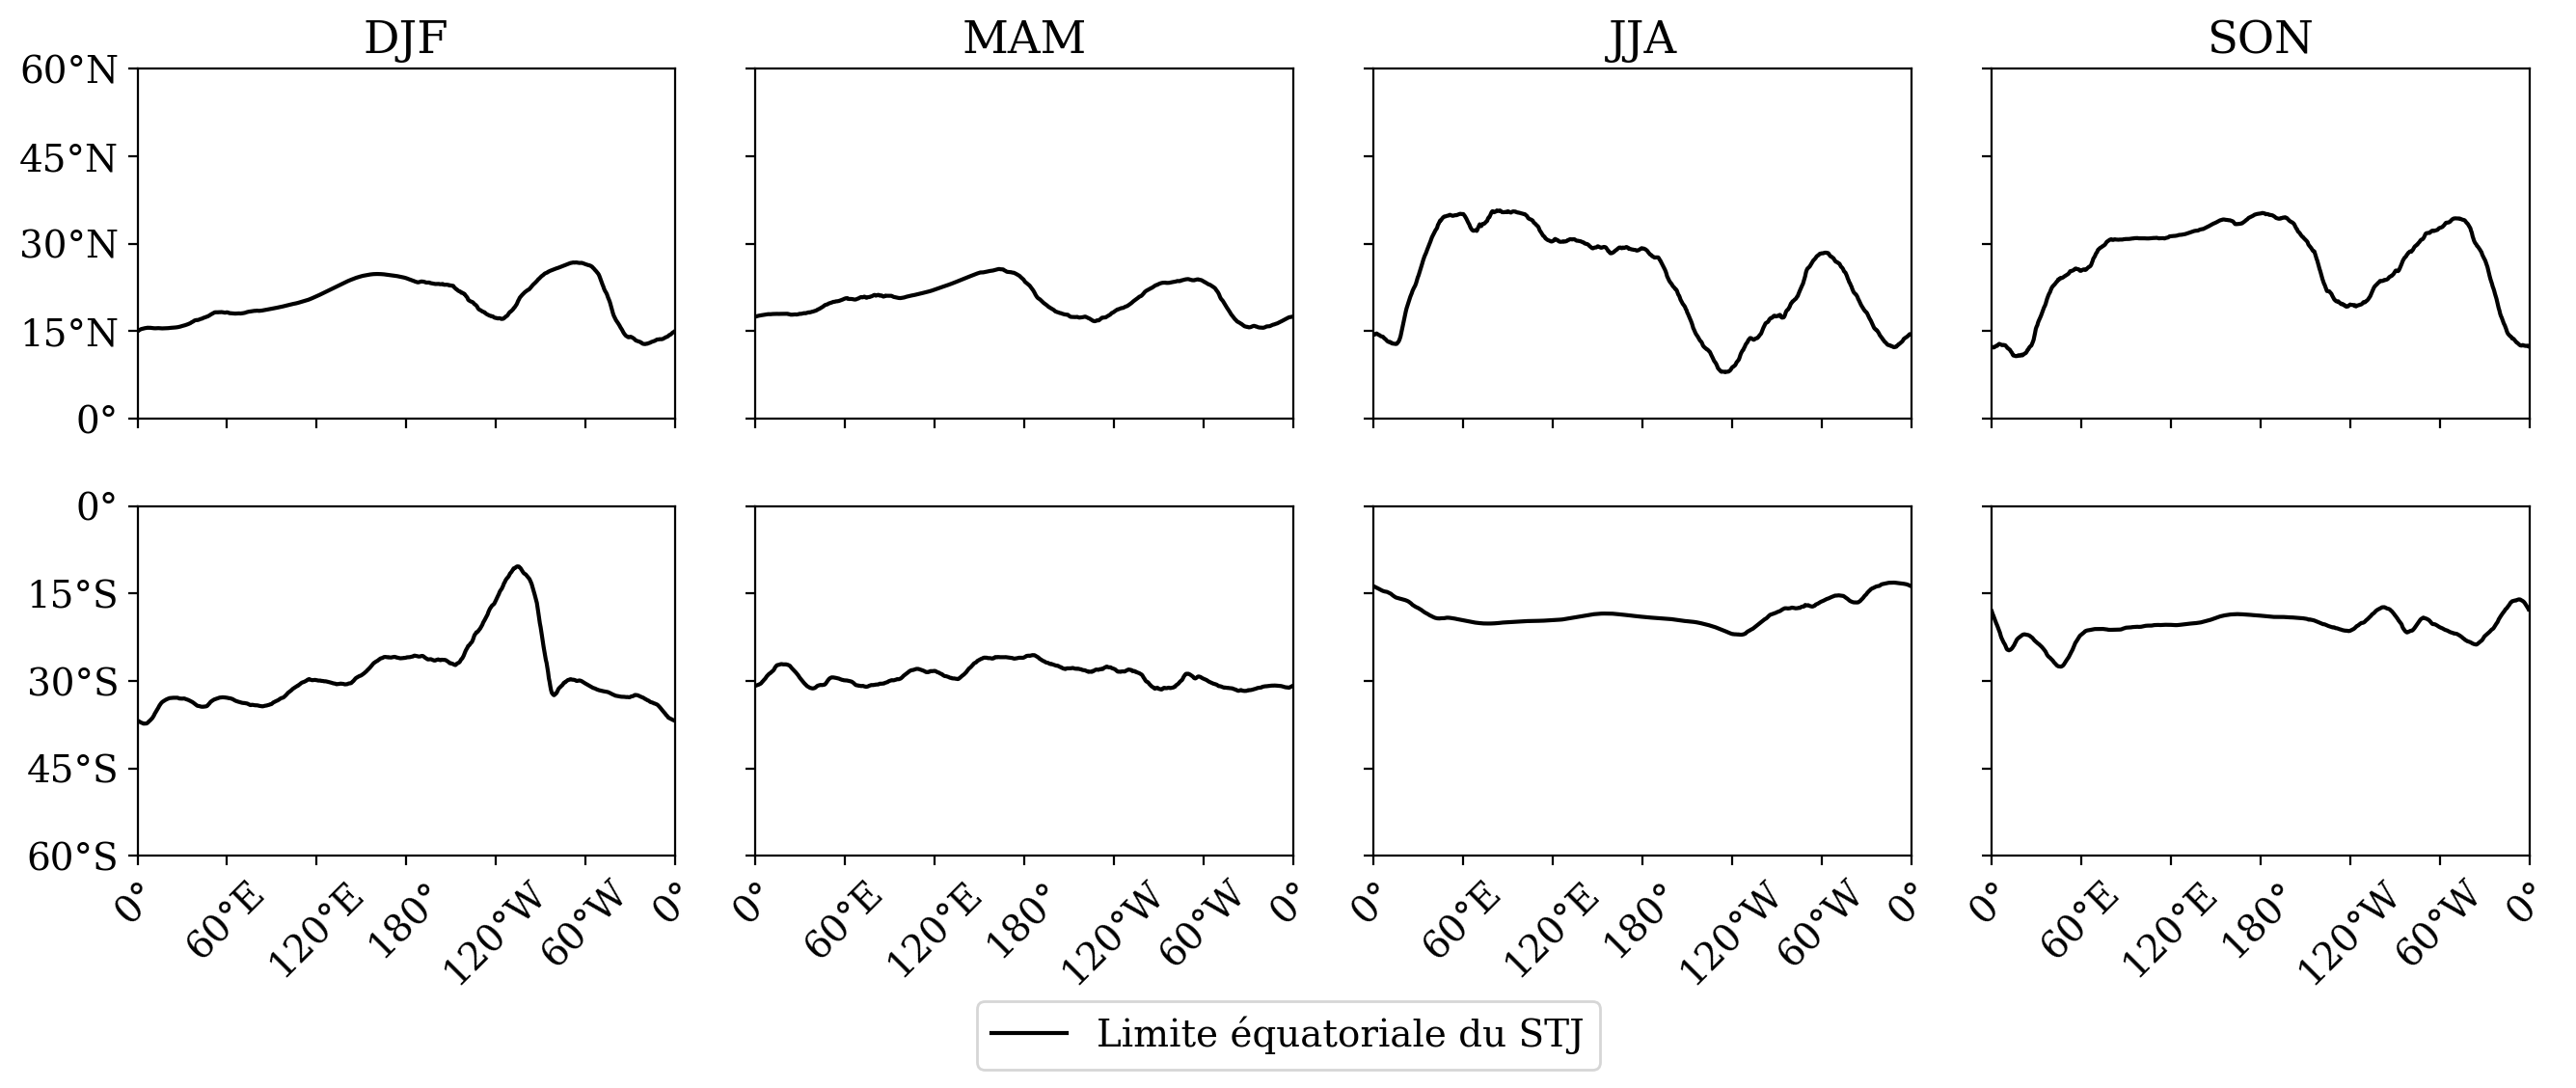
\includegraphics[width=\textwidth]{STJ_season_PRE625REFT359x.png}
%    \caption{Moyennes saisonnières de la latitude de la limite équatoriale du jet subtropical dans la simulation ARPEGE-Climat forcée par HadISST1. Chacune des
%    quatre colonnes correspond à une saison. La première ligne présente le diagnostique pour l'hémisphère nord, tandis que la seconde ligne le présente pour
%    l'hémisphère sud.}
%    \label{fig:STJ_PRE625REFT359x}
%\end{figure}

\subsubsection{Diagnostique ENSO}\label{sec:diag_enso}

Le mode de variabilité El Niño (respectivement El Niña) est caractérisé par une anomalie chaude (respectivement froide) de SST dans l'oćean Pacifique central.
Il existe plusieurs façons de diagnostiquer ce phénomène et qui se distinguent entre elles par la région, ou boîte, utilisée pour calculer l'anomalie de
température, ainsi que par le lissage temporel utilisé. Ces boîtes sont au nombre de \num{4}, réparties entre les côtes de l'Amérique centrale et les îles
Salomon. L'anomalie de SST prise dans une de ces boîtes définit alors un indice El Niño. Ici, nous utilisons l'indice ENSO utilisé pour les besoins
opérationnels de la NOAA, nommé ONI (\textit{Oceanic Niño Index}). L'ONI est définit sur la boîte 3.4, c'est à dire à cheval sur les boîtes \num{3} et \num{4}
(non montrées) et définie entre \ang{120}W et \ang{170}W, et entre \ang{5}S et \ang{5}N. Les anomalies sont lissées sur \num{3} mois glissants, et la référence
climatologique est prise comme la SST moyenne sur la toute la période disponible. La \cref{fig:ONI} présente la boîte 3.4 utilisée pour calculer l'anomalie de
température, ainsi que la série temporelle de l'ONI entre janvier \num{1980} et décembre \num{2010}.

\begin{figure}[htpb]
    \centering
    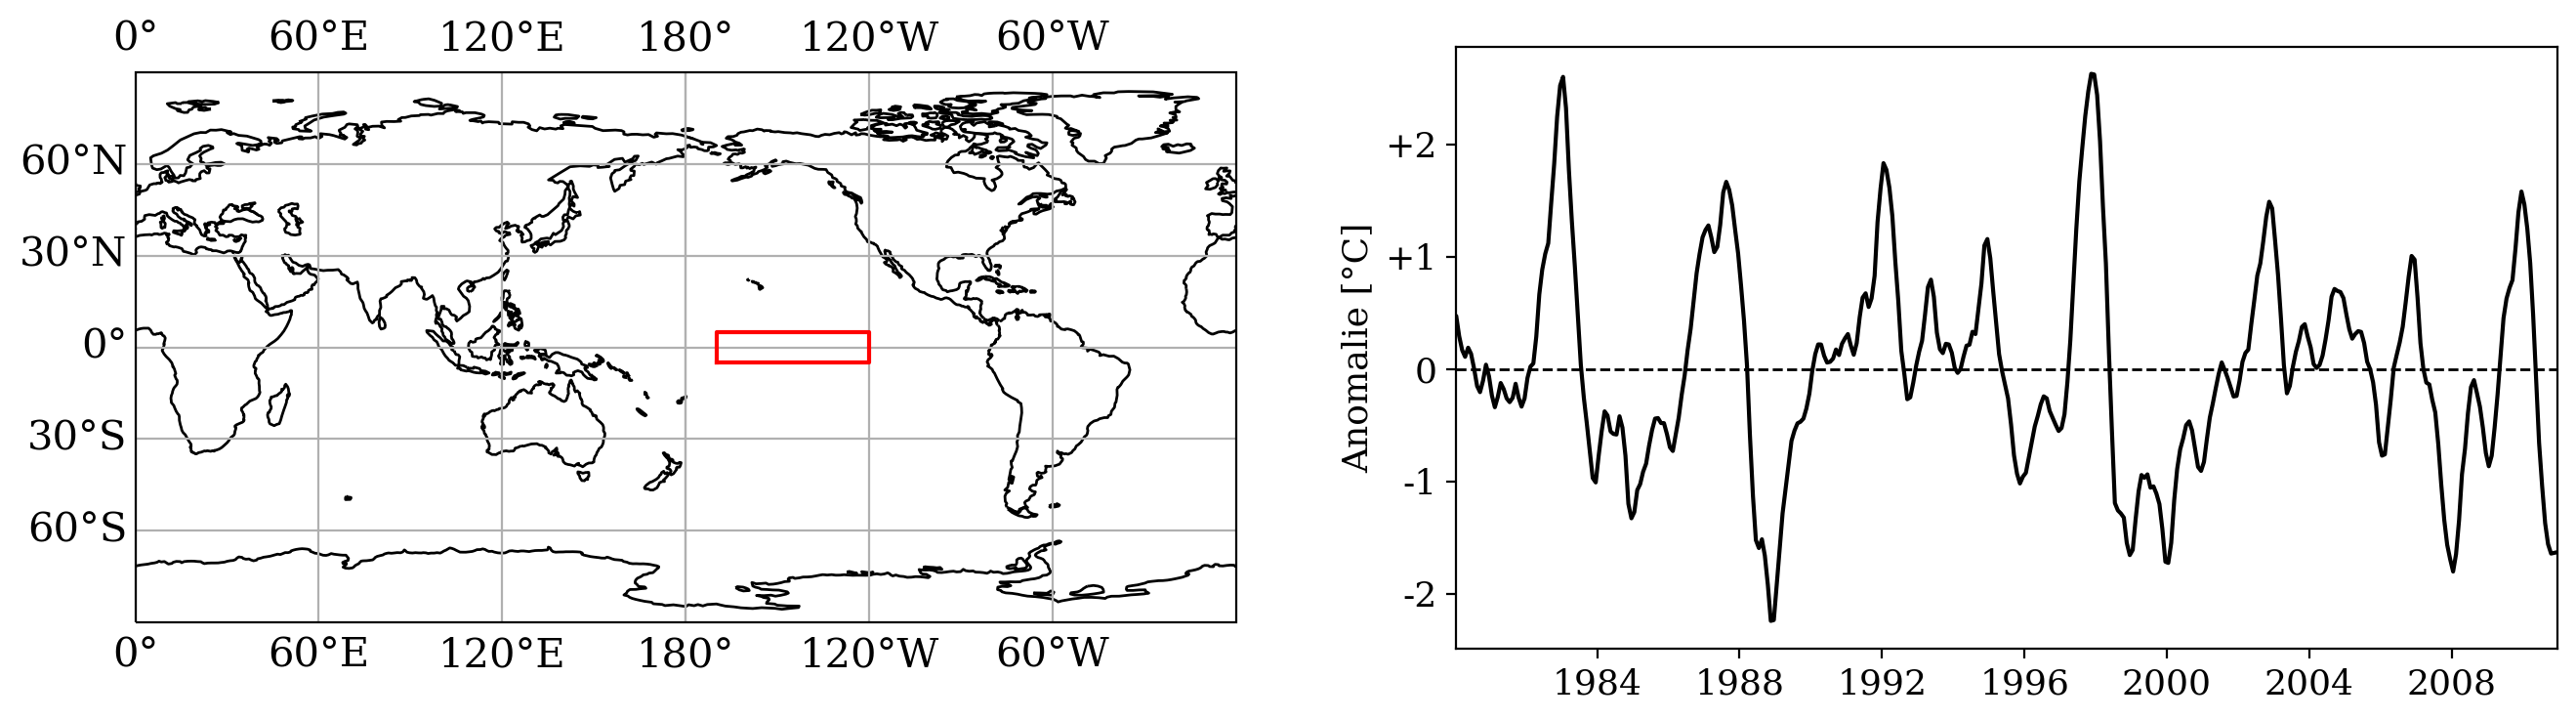
\includegraphics[width=\textwidth]{ONI.png}
    \caption{Boîte 3.4 utilisée pour le calcul de l'ONI (gauche) et série temporelle de l'ONI (droite) évaluée sur la SST mensuelle de la
    simulation ARPEGE forcée par HadISST1.}
    \label{fig:ONI}
\end{figure}

Pour utiliser l'ONI comme prédicteur dans une régression de Poisson, il est nécessaire de le transformer en vecteur de la même taille $m$ (c.f
\cref{chap:chapitre_3}, \cref{sec:regression_poisson}) que les champs spatio-temporels de grande échelle. L'ONI étant, pour un mois donné, un scalaire ; sa
valeur est répliquée en tout point de la grille spatiale souhaitée. Cela revient à considérer que chaque point de l'espace a connaissance à chaque
pas de temps de l'anomalie de SST dans la boîte 3.4.

\subsection{Lien entre ENSO et l'activité cyclonique dans ARPEGE}\label{sec:lien_enso_tracking}

Le lien entre ENSO et l'activité cyclonique tropicale dans les observations et dans les modèles est largement documenté
\parencite{chan_tropical_1985,wu_gcm_1992,landsea_ninosouthern_2000,mcdonald_tropical_2005,lin_enso_2020}. Une phase positive de l'oscillation El-Niño tend à
augmenter la fréquence d'occurence des TC dans certains bassins, notamment dans le Pacifique, et tend à la réduire dans l'océan Indien, et vice versa. Dans
l'Atlantique nord, l'activité cyclonique est traditionnellement anti-corrélée à ENSO, car ce dernier apporte du cisaillement dans l'océan Atlantique. Cependant,
pour déterminer dans quelle mesure l'ajout de l'ONI comme prédicteur dans une régression établie sur les cyclogénèses détectées dans le modèle ARPEGE peut impacter la
fréquence statistiquement modélisée, il convient de quantifier le lien entre l'ONI et l'activité cyclonique dans notre jeu de données.

La \cref{fig:corr_ONI_pt} présente la carte de corrélation entre le nombre annuel de cyclogénèses pour chaque maille d'une grille régulière de \ang{3} de
résolution et l'ONI, aggrégé annuellement de la même façon. Précisons que, à l'instar de toutes les opérations de calcul de variabilité interannuelle
réalisées jusqu'à maintenant, et notamment dans le \cref{chap:chapitre_3}, la fréquence annuelle est calculée pour les saisons cycloniques. Dans l'hémisphère
sud, le nombre de TC pour une saison donnée est donc évalué entre juillet de l'année précédente et juin de l'année courante. Précisons aussi qu'un masque
terre-mer interpolé sur la grille de \ang{3} de résolution est utilisé pour masquer les cyclogénèses détectées sur terre de la
\cref{fig:track_density_PRE625REFT359x}.

\begin{figure}[tpb]
    \centering
    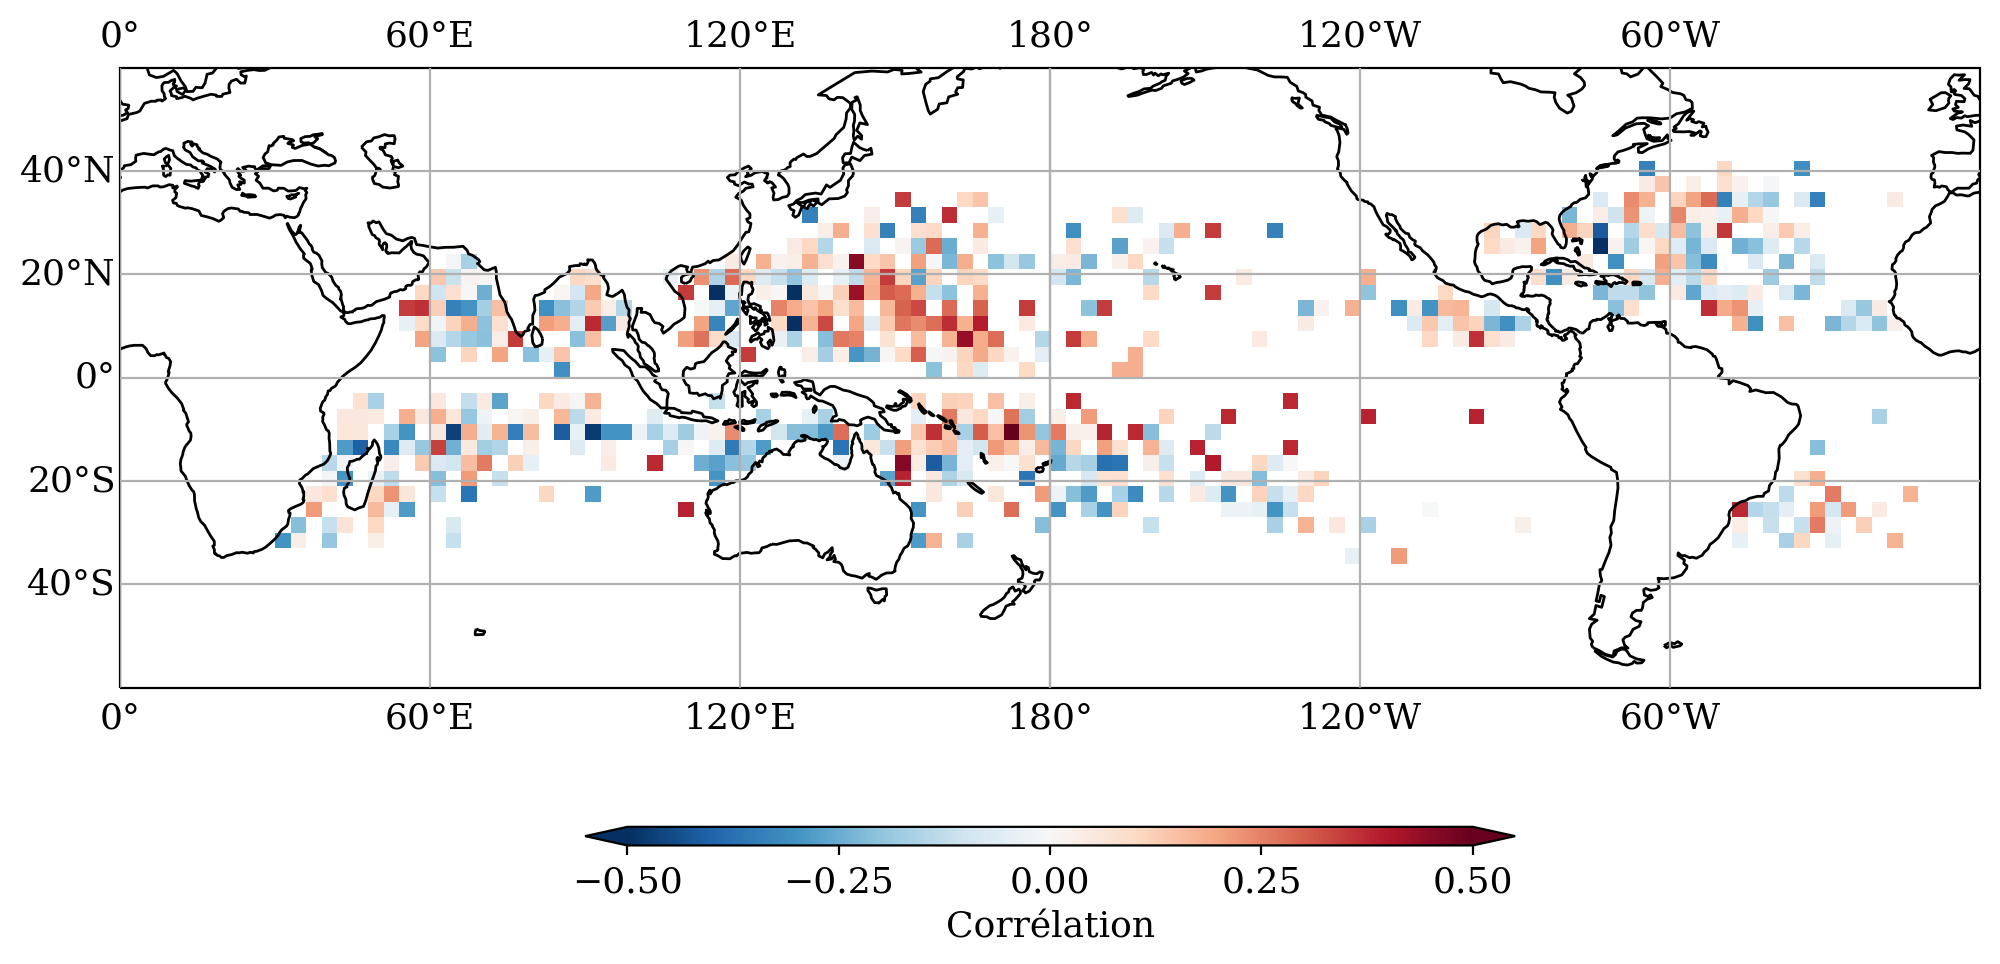
\includegraphics[width=\textwidth]{corr_ONI_tracks.png}
    \caption{Carte de corrélation entre la variabilité interannuelle de l'activité cyclonique par point de grille (\ang{3}x\ang{3}) pour les cyclogénèses
    détectées dans ARPEGE et l'ONI, sur les saisons cycloniques entre \num{1980} et \num{2010}.}
    \label{fig:corr_ONI_pt}
\end{figure}

La \cref{fig:corr_ONI_pt} met en évidence des corrélations contrastées dans les différents bassins d'activité. Le signal le plus clair est noté dans le WPac, à
l'ouest de \ang{180}, avec une corrélation positive dans la plupart des mailles où des cyclogénèses ont été détectées. Certaines dépassent la borne supérieure
de la carte des couleurs fixée à \num{0.5}. Dans le bassin EPac, le peu de cyclogénèses disponibles (voir
\cref{fig:track_density_PRE625REFT359x,fig:density_arpege_ibtracs}) empêche l'interprétation de la corrélation. Dans le SPac, des corrélations positives
relativement fortes sont notées dans la partie nord, tandis que ces dernières s'inversent au delà de \ang{20}S. Dans le bassin SIndE, ENSO apparaît clairement
anti-corrélée à l'activité cyclonique, à l'exception de quelques mailles. Pour les bassins SIndW NInd et NAtl, le signal est plus contrasté mais laisse également
entrevoir dans l'ensemble une possible anti-corrélation.

Pour évaluer le lien entre l'activité cyclonique détectée et la variabilité El Niño dans ces bassins où la \cref{fig:corr_ONI_pt} ne permet pas de dégager une
conclusion nette, la corrélation est évaluée à l'échelle du bassin tout entier. Spécifiquement, les cyclogénèses sont comptabilisées sur la grille d'origine de
la simulation (T359, soit \ang{0.5}), puis l'activité est intégrée spatialement sur les bassins océaniques usuels selon la méthodologie employée dans le
\cref{chap:chapitre_3}. Enfin, la corrélation avec la variabilité interannuelle de l'ONI est évaluée pour chacun des bassins. La
\cref{fig:corr_ONI_bassin} présente les coefficients de corrélation $r$ ainsi que les valeurs-p associées.

\begin{figure}[tpb]
    \centering
    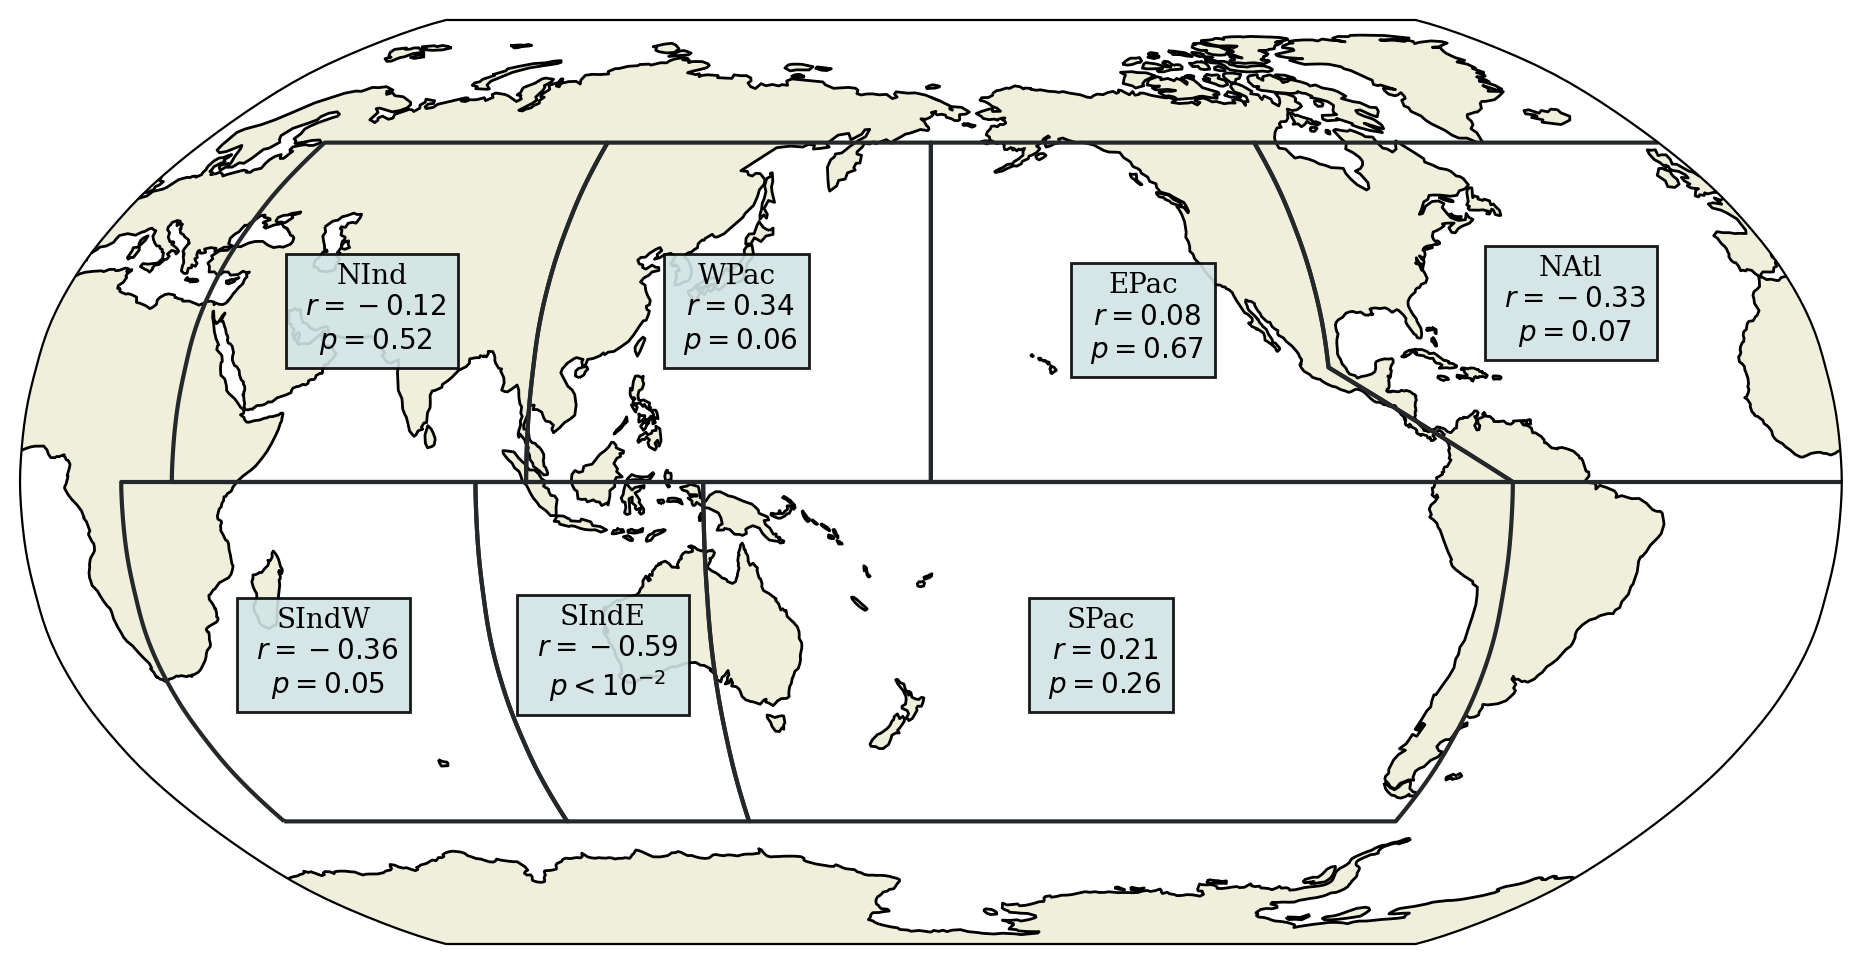
\includegraphics[width=\textwidth]{corr_ONI_bassin}
    \caption{corrélation entre la variabilité interannuelle de l'activité cyclonique détectée dans ARPEGE et l'ONI à l'échelle des bassins océaniques.}
    \label{fig:corr_ONI_bassin}
\end{figure}

Pour les bassins WPac et SIndE, la \cref{fig:corr_ONI_bassin} confirme ce que laisse deviner la \cref{fig:corr_ONI_pt}, à savoir une corrélation dans le
premier, évaluée à \num{0.34} et à la limite de la significativité sous un seuil de \prct{95}, et une anti-corrélation significative dans le second à
\num{-0.59}. La \cref{fig:corr_ONI_bassin} permet également de lever l'ambigüité pour les bassins où le lien est contrasté sur la \cref{fig:corr_ONI_pt}. Ainsi
l'activité cyclonique dans le bassin SIndW est également présenté comme anti-corrélée à l'ONI avec \num{-0.36}, là aussi à la limite de la significativité, et
pareillement dans le bassin NAtl avec \num{-0.33}, bien qu'avec une valeur-p de \num{0.07}. En revanche, le bassin EPac ne présente aucune corrélation, et
celles des bassins NInd et SPac ne sont pas significatives. À titre de référence, cette carte réalisée entre ERA5 et IBTrACS signale une corrélation de
\num{0.54} dans le bassin EPac et de \num{-0.43} dans le bassin NAtl. La corrélation dans le bassin SIndE est inchangée par rapport à celle mesurée ici, mais
les bassins WPac et SIndW sont néanmoins parfaitement décorrélés.

Le lien entre l'activité cyclonique telle que détectée par le schéma de détection du CNRM appliqué au modèle ARPEGE d'une part, et le mode de variabilité El
Niño est dans l'ensemble cohérent. Plusieurs bassins océaniques présentent des corrélations à la limite de la significativité statistique, et c'est par
conséquent dans ces bassins là qu'une éventuelle plus-value de l'ajout de l'ONI comme prédicteur dans une régression de Poisson peut être attendue.

\subsection{Application de la régression}

On applique ici la régression de Poisson selon la même méthodologie employée pour construire l'indice nommé M10 dans la \cref{sec:apport_res_temporel_spatial},
mais appliquée à la simulation ARPEGE. On utilise donc en prédictant les cyclogénèses détectées par le traqueur du CNRM dans la simulation historique ARPEGE
forcée par HadISST1. Ces dernières, de même que les champs de grande échelle utilisés comme prédicteurs, transposées sur une grille régulière de \ang{1} de
résolution et agrégées au pas de temps mensuel. Ici encore, la taille de la matrice $\mathbf{x}$ des prédicteurs est le principal facteur limitant la résolution
spatiale pour réaliser la régression, et est la raison pour laquelle nous n'utilisons pas la grille T359 d'origine. Nous utilisons les mêmes variables
thermiques et dynamiques que pour le TCS et pour les \cref{sec:apport_res_temporel_spatial,sec:indice_regional}, à savoir la vorticité absolue bornée à
\SI{3.7e-5}{\per\second} $\eta$, le cisaillement vertical $V_{\mathrm{shear}}$ entre \hPa{850} et \hPa{200}, l'humidité relative $H$ à \hPa{600} et la SST
relative $T$.

Nous définissons dans un premier temps l'équivalent de l'indice M10 pour ARPEGE, nommé AM10. Nous réalisons ensuite une seconde régression en ajoutant à
ces quatre variables décrivant l'environnement de grande échelle le champ artificiel de l'ONI, définit en tout point de la grille comme l'anomalie
mensuelle de SST dans la boîte 3.4 présentée dans la \cref{sec:diag_enso}. L'indice incluant l'ONI comme prédicteur est nommé OAM10, abrégé en OA. La régression
avec l'ONI comme prédicteur est appliquée aussi bien à l'échelle globale qu'à l'échelle des bassins individuels. Dans le second cas, la méthodologie employée
dans la \cref{sec:indice_regional} pour construire l'indice LM10 est transposée aux prédicteurs et prédictant ARPEGE, notamment pour ce qui concerne la
calibration de l'indice régional sur la fréquence annuelle moyenne inférée par son homologue global. L'indice régional est alors nommé LOAM10, ou simplement
LOA, puisqu'il est entendu que, contrairement au \cref{chap:chapitre_3}, les régressions sont uniquement faites avec les moyennes mensuelles à \ang{1} de
résolution.

Enfin, précisons que les cyclogénèses détectées sur terre sont masquées, si bien que la fréquence annuelle de référence pour la calibration des indices globaux
est réduite à \num{52.32} TC par an. Bien que ce nombre soit bien différent de la fréquence de référence issue IBTrACS utilisée dans le \cref{chap:chapitre_3},
cela n'a aucune importance dès lors que tous les indices sont calibrés sur cette valeur. Le TCS de \textcite{tippett_poisson_2011} est également pris comme
référence pour la comparaison des résultats.

\subsubsection{Régressions globales}

Nous nous intéressons dans un premier temps aux coefficients obtenus pour les régressions globales AM10 et OAM10. L'indice de cyclogénèse AM10 est donné
ci-dessous :
%
\begin{align*}
\tag{AM10}
    \mu &= \exp \big( b_0 + b_\eta \eta + b_{V_{\mathrm{shear}}} V_{\mathrm{shear}} + b_H H + b_T T + \log \cos \phi \big)\\
        &= \exp \big( \num{-18.6861} + \num{2.4363} \eta - \num{0.0192} V_{\mathrm{shear}} + \num{0.0454} H + \num{0.4202} T + \log \cos \phi \big)
\end{align*}
%
Les coefficients de AM10 sont à mettre en regard avec ceux obtenus pour l'indice M10, obtenus entre ERA5 et IBTrACS dans le \cref{chap:chapitre_3}. Ces derniers
peuvent être consultés dans le \cref{tab:fit_spatial_temporel}, \vpageref{tab:fit_spatial_temporel}. Le coefficient $b_H$ est réduit d'environ \num{0.072} à
\num{0.045}, soit une valeur proche du coefficient associé à l'humidité relative du TCS (\num{0.05}). Les coefficients $b_T$ sont quant à eux quasi identiques,
à \num{0.01} près. Cela peut vraisemblablement s'expliquer par le fait que la réanalyse ERA5 assimile des données la SST issue de la base de données HadISST2
jusqu'en \num{2007}. La sensibilité au cisaillement vertical est néanmoins réduite dans AM10, passant d'environ \num{-0.1} dans ERA5 à environ \num{-0.02} dans
ARPEGE, soit une sensibilité cinq fois moindre dans le modèle de climat. Cette valeur du coefficient apparaît néanmoins comme statistiquement significative
(ainsi que tous les autres coefficients) en dépit de sa valeur proche de \num{0}. La régression indique en effet des pourcentiles \prct{2.5} et \prct{97.5} de
respectivement \num{-0.027} et \num{-0.011} pour $b_{V_{\mathrm{shear}}}$, et une valeur-p inférieure à \num{1e-3}. Le coefficient associé à la vorticité
absolue est celui présentant la plus grande différence pasant d'environ \num{1.40} pour M10 à \num{2.44} pour AM10. Une valeur si élévée de $b_\eta$ est
cohérente avec le biais septentrional dans les cyclogénèses détectées dans ARPEGE (voir \cref{fig:density_arpege_ibtracs}), puisqu'il a été largement montré
dans le \cref{chap:chapitre_3} que des valeurs élevées de ce paramètre sont associées à une activité simulée par la régression plus éloignée de l'équateur.

La relation pour l'indice OA est donnée ci-dessous :
%
\begin{align*}
    \tag{OA}
    \mu &= \exp \big( b_0 + b_\eta \eta + b_{V_{\mathrm{shear}}} V_{\mathrm{shear}} + b_H H + b_T T + b_{\mathrm{ONI}} \mathrm{ONI} + \log \cos \phi \big)\\
        &= \begin{aligned}[t]\exp \big( \num{-18.7099} + \num{2.4430}\, \eta - \num{0.0192}\, V_{\mathrm{shear}} + &\num{0.0454}\, H + \num{0.4221}\, T + \\&\underbrace{\num{0.0638}\, \mathrm{ONI}}_{\mathrm{Indice\ ENSO}} + \log \cos \phi \big)\end{aligned} \end{align*}
%
L'ajout de l'ONI dans la régression ne modifie que très marginalement les coefficients associés aux autres prédicteurs. On ne note qu'une très légère hausse de
$b_\eta$ ainsi qu'une augmentation toute aussi faible de $b_T$. La régression indique cependant une sensibilité positive à l'ONI avec une valeur
$b_{\mathrm{ONI}}$ d'environ \num{0.06}. Cela signifie qu'à l'échelle globale, un changement de $+$\SI{1}{\degreeCelsius} de l'anomalie de SST dans la région
3.4 provoque une hausse de la fréquence d'occurrence modélisée par la régression de l'ordre \prct{6}. Cette valeur apparaît comme statistiquement significative,
avec une valeur-p de \num{0.024}. Il s'agit toutefois de la valeur-p la plus élevée notée jusqu'à maintenant, ces dernières étant sinon systématiquement
inférieures à \num{1e-3}, pour toutes les régressions réalisées dans le \cref{chap:chapitre_3} et dans le chapitre présent. La régression indique un AIC
\parencite[\textit{Akaike Information Criterion},][]{akaike_information_1998} ---~c'est à dire une log-vraisemblance ajustée par le nombre de prédicteurs~---
légèrement réduite par rapport à AM10, passant en effet de \num{24752} à \num{24747}, indiquant une régression de qualité légèrement supérieure lorsque la
variable ONI est introduite.

Néanmoins, la \cref{sec:lien_enso_tracking} montre que le lien entre ENSO et l'activité cyclonique n'est pas uniforme dans l'espace, avec certaines régions
exprimant une corrélation positive, et d'autres une anti-corrélation. Un indice de cyclogénèse formulé sur l'ONI et dont la régression est menée à l'échelle
globale ne peut donc satisfaire le rapport entre ce mode de variabilité et l'activité constatée dans tous les bassins. Sachant cela, il est permis de penser que
le signe positif de $b_{\mathrm{ONI}}$ pour AM10 et sa significativité statistique sont fortement influencés par le bassin WPac, présentant sur la
\cref{fig:corr_ONI_bassin} une corrélation positive, et influençant d'avantage la régression en sa qualité de bassin le plus actif. C'est pour cette raison que la
régression est répétée à l'échelle des bassins.

\subsubsection{Régressions locales}

Le \cref{tab:coefs_LOA} présente les coefficients obtenus pour chacune des régressions faites à l'échelle des bassins océaniques. On s'intéresse tout
particulièrement aux coefficients associés à l'ONI, aux intervalles de confiance ainsi qu'à la significativité de l'ajout de ce prédicteur dans l'indice LOA.

\begin{table}[htpb]
    \centering
    \caption{Coefficients estimés des prédicteurs pour les régressions réalisées à l'échelle des bassins océaniques avec l'ONI. Les pourcentiles \prct{2.5},
    \prct{97.5} des valeurs de $b_{\mathrm{ONI}}$ sont données, de même que la valeur-p pour ce coefficient. La colonne Fréquence indique le nombre de TC par an
    dans chacun des bassins. Chaque indice régional est calibré sur la fréquence annuelle moyenne de l'indice OA pour ce bassin.}
    \label{tab:coefs_LOA}
    \resizebox{\textwidth}{!}{
    \begin{tabular}{lrrrrrrrrrr}
       \toprule\toprule 
       \multicolumn{1}{c}{Bassin} & \multicolumn{6}{c}{Coefficients} & \multicolumn{3}{c}{ONI} & \multicolumn{1}{c}{Fréquence}\\
       \midrule
                                  & $b_0$ & $b_{\eta}$ & $b_{V_{\mathrm{shear}}}$ & $b_H$ & $b_T$ & $b_{\mathrm{ONI}}$ & \prct{2.5} & \prct{97.5} & valeur-p \\
       \midrule
       NAtl    & \num{-16.7188} & \num{2.3260} & \num{-0.0467} & \num{0.0219} & \num{0.3147} & \num{-0.0737} & \num{-0.237} & \num{0.089} & \num{0.376} & \num{6.41} \\
       WPac    & \num{-17.2232} & \num{1.9807} & \num{-0.0321} & \num{0.0501} & \num{0.3457} & \num{0.2184} & \num{0.116} & \num{0.321} & $< 10^{-3}$ & \num{19.40} \\
       EPac    & \num{-16.9821} & \num{2.0161} & \num{-0.0434} & \num{0.0352} & \num{0.3874} & \num{0.0790} & \num{-0.192} & \num{0.350} & \num{0.568} & \num{5.54} \\
       NInd    & \num{-19.9302} & \num{2.8346} & \num{-0.0450} & \num{0.0624} & \num{0.2984} & \num{0.0559} & \num{-0.081} & \num{0.193} & \num{0.425} & \num{3.98} \\
       SPac    & \num{-19.5598} & \num{2.8841} & \num{-0.0397} & \num{0.0340} & \num{0.4375} & \num{0.1797} & \num{0.053} & \num{0.306} & \num{0.005} & \num{10.12} \\ 
       SIndW   & \num{-17.8103} & \num{2.4274} & \num{-0.0367} & \num{0.0385} & \num{0.3672} & \num{-0.1257} & \num{-0.281} & \num{0.030} & \num{0.113} & \num{3.96} \\
       SIndE   & \num{-19.3702} & \num{3.0105} & \num{-0.1024} & \num{0.0403} & \num{0.4964} & \num{-0.1164} & \num{-0.304} & \num{0.071} & \num{0.224} & \num{2.09} \\
       \bottomrule
    \end{tabular}
    }
\end{table}

Les bassins NInd et EPac présentent les valeurs-p associées à leur coefficient $b_{\mathrm{ONI}}$ les plus élevées de toutes, jusqu'à \num{0.568} pour ce
dernier. Ces mêmes bassins présentaient également les liens les moins prononcés entre ENSO et la variabilité interannuelle dans la
\cref{sec:lien_enso_tracking}. Dans le bassin NAtl, la variable ONI apparait non-significative avec une valeur-p de \num{0.376}. Le coefficient
$b_{\mathrm{ONI}}$, valant environ \num{-0.07}, reflète toutefois le signe du coefficient de corrélation de la \cref{fig:corr_ONI_bassin}, et l'intervalle de
confiance ---~bien que traversant le \num{0}~--- est clairement plus situé du côté des valeurs négatives que des valeurs positives, avec des quantiles
\num{0.025} et \num{0.975} de respectivement \num{-0.237} et \num{0.089}. Un constat similaire peut être fait pour les bassins SIndW et SIndE. Les valeurs-p y
sont en effet supérieures à \num{0.05}, mais leurs coefficients, de respectivement \num{-0.13} et \num{-0.12}, de même que leur intervalle de confiance exprimé
par les pourcentiles \prct{2.5} et \prct{97.5}, sont cohérents avec les résultats de la \cref{fig:corr_ONI_bassin}. Notons que des deux bassins, le SIndW
présente la valeur-p la plus faible à \num{0.113}. Enfin, les régressions faites dans les bassins SPac et WPac acceptent toutes deux le prédicteur ONI, avec une
valeur-p $\leq$ \num{0.05}, bien que le premier soit en limite de significativité. Le coefficient $b_{\mathrm{ONI}}$ dans le bassin WPac est par ailleurs le
plus élevé de tous avec \num{0.22}. Cela conforte la suspicion selon laquelle ce bassin influence fortement le signe du coefficient dans l'indice global OA. Il
convient de noter que la significativité dans le bassin SPac d'une part, et la non-significativité dans les bassins SIndW et SIndE n'étaient pas nécessairement
attendues, puisque la \cref{fig:corr_ONI_bassin} fournit l'information inverse. 

Ainsi, les valeurs prises dans les différentes régions par le coefficient $b_{\mathrm{ONI}}$ reflètent, au moins par leur signe, le lien présenté entre la
variabilité El Niño et l'activité cyclonique détectée dans la simulation ARPEGE forcée, en dépit d'une significativité peu franche, à l'exception notable du
bassin WPac. L'alternance entre le signe du coefficient justifie néanmoins la construction d'indices régionaux plutôt que globaux pour l'ajout de prédicteurs
dont l'effet sur l'activité cyclonique n'est pas uniforme dans toutes les régions du monde.

\subsubsection{Variabilité interannuelle}

La \cref{fig:variability_ONI} présente les variations du nombre de TC d'une saison cyclonique à l'autre pour les trois indices établis sur la simulation ARPEGE
historique, pour le TCS ainsi que vue par le schéma de détection du CNRM. Rappelons que, à l'instar de la \cref{sec:indice_regional} du
\cref{chap:chapitre_3}, l'indice LOA est en fait défini par un indice régional différent pour chaque bassin, dont les coefficients sont donnés dans le
\cref{tab:coefs_LOA}. La variabilité temporelle du nombre de TC détectés dans ARPEGE par le traqueur du CNRM est noté \textquote{Tracks}.

\begin{figure}[p]
    \centering
    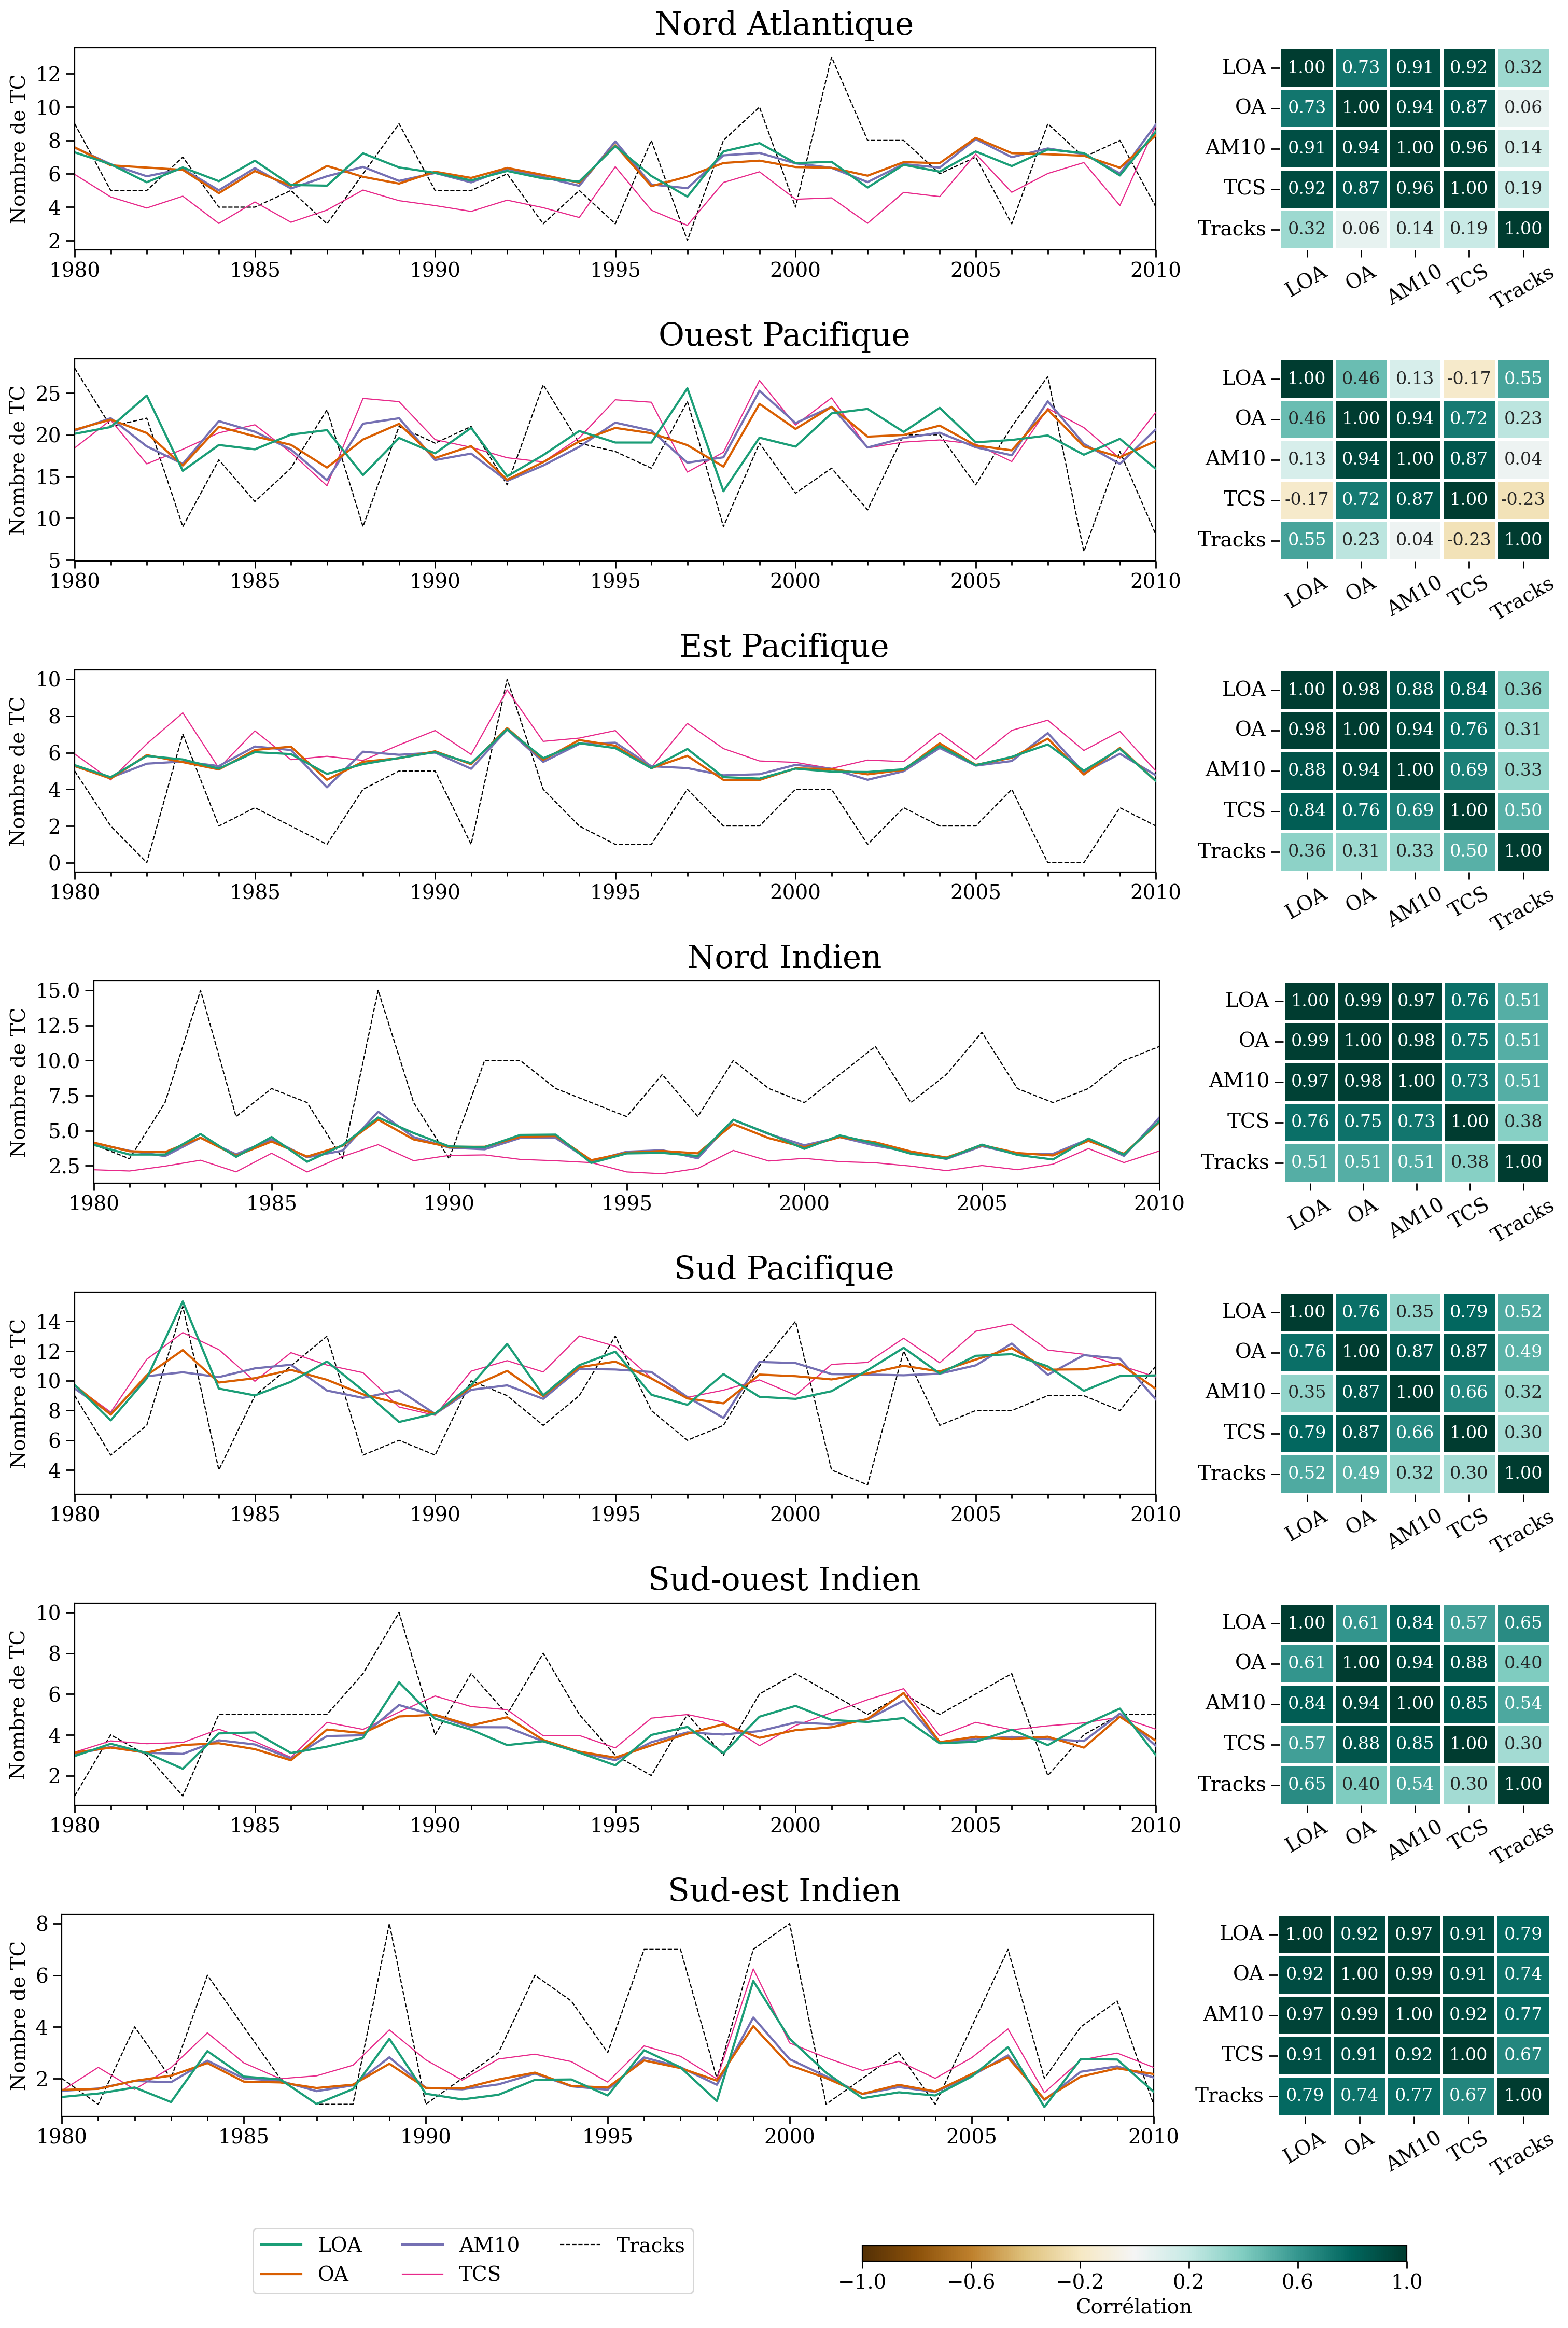
\includegraphics[height=0.94\textheight]{basin_variability_LOA_OA_AM10_TCS_Obs.png}
    \caption{Variabilité interannuelle des trois indices construits sur la simulation ARPEGE, du TCS et issue du schéma de détection (Tracks), ainsi que les
    matrices de corrélation associées.}
    \label{fig:variability_ONI}
\end{figure}

\subsection{Conclusion}

Les résultats obtenus dans le \cref{chap:chapitre_3} tendent à montrer que la régression de Poisson vise avant tout à fournir la meilleure vraisemblance
spatiale, sans garantie sur la variabilité temporelle. Ainsi, la non-significativité du prédicteur dans les régressions locales peuvent se comprendre par le
fait que l'ONI n'améliore pas la répartition spatiale de l'activité inférée par l'indice, mais ne présage pas nécessairement néanmoins apporter une

\section{Tendances}

%--------------------------------------
\section{Synthèse}

\end{document}
